\chapter{Amplificadores Operacionales}
 
 
 \hspace{10pt} \textbf{ Ejercicio 1}:  Dado el circuito de la figura \ref{op1} hallar una expresión general del desajuste de salida en función de $V_{OS}$, $I_{OS}$  e $I_B$ . Indique posibles soluciones para contrarrestar los desajustes. Evaluar la
expresión hallada en los siguientes casos, resaltando en ellos cuál es el parámetro que puede ser
medido: a)  $R_1 =\infty$   , $R_2 = R_3 = 0$; b)  $R_1 =\infty$, $R_2 = 10 M\Omega$ , $R_3 =
0$; c)  $R_1 = \infty$, $R_2 = 0$, $R_3 = 10 M\Omega$; d)  $R_1 = \infty$, $R_2 = R_3 = 10 M\Omega$.



\textbf{Ejercicio 2}: En el circuito de la figura \ref{op2}, obtener
la tensión de desajuste de salida y su corrimiento con la
temperatura si $V_{OS} = 1 mV$, $I_B = 70 nA$ , $I_{OS} = 10 nA$ ,
$\displaystyle \frac{\Delta V_{OS}}{\Delta T}= 10 \mu V/°C$ ,
$\displaystyle \frac{\Delta I_{OS}}{\Delta T}= 10 pA/°C$ y
$\displaystyle \frac{\Delta I_{B}}{\Delta T}= 1  nA/°C$.



\textbf{Ejercicio 3}: En el circuito de la figura \ref{op3}, hallar:
a)  $\displaystyle \frac{v_o}{(v_1-v_2)}$ y b)  máximo desajuste de
salida



\textbf{Ejercicio 4}: Dado el circuito de la figura \ref{op4}
hallar: a) $\displaystyle \frac{V_o}{(V_1-V_2)}$. b) Máximo
desajuste de $V_o$ en función de $V_{OS}$, $I_{OS}$ e $I_B$,
suponiendo los operacionales iguales.



\textbf{Ejercicio 5}:  Explicar el funcionamiento de las
aplicaciones de amplificadores operacionales mostradas en la figura
\ref{op5}.


\textbf{Ejercicio 6}: En la figura \ref{op6} se ilustra un filtro
pasabanda activo RC de segundo orden. Hallar la transferencia
$A_v(s)=\displaystyle \frac{V_o(s)}{V_i(s)}$. Escribir la ecuación
de ganancia de tal modo que en el denominador aparezca un polinomio
de segundo grado en s y por analogía con la impedancia de un
circuito resonante paralelo RLC, calcular el factor de calidad Q y
el ancho de banda. Hallar el valor de frecuencia central o de
resonancia.

Impedancia de un circuito RLC paralelo: $Z(s)=\displaystyle
\frac{\displaystyle \frac{s}{C}}{s^2+\displaystyle
	\frac{s}{RC}+\displaystyle \frac{1}{LC}}$


\textbf{Ejercicio 7}: El circuito mostrado en la figura \ref{op7} es
un convertidor de impedancia negativa. Calcule la impedancia de
entrada. Verifique la condición de estabilidad: $R_g \times R_2
> R_1 \times R_L$ .


\textbf{Ejercicio 8}: Dado el circuito de la figura \ref{op8}
determinar $\displaystyle \frac{I_L}{(V_1-V_2)}$. ¿Qué ocurre si
$Z_L$ es un capacitor?


\textbf{Ejercicio 9}: El circuito de la figura \ref{op9} es un
conversor CA/CC de precisión , que permite obtener, además el valor
medio de la señal rectificada. Explicar el funcionamiento.



\textbf{Ejercicio 10}: Para cada etapa del circuito de la figura
\ref{op10} determinar: a) Funcionamiento. b)  Formas de onda.



\textbf{Ejercicio 11}:  En el circuito de la figura \ref{op11}
hallar el valor de $R_4$, tal que ocasione un $Q = 50$.



\textbf{Ejercicio 12}: En el circuito de la figura \ref{op12},
hallar la forma de onda de salida (amplitud y frecuencia).






\textbf{Ejercicio 13}; En el circuito de la figura \ref{op13} hallar
la curva de transferencia.


\textbf{Ejercicio 14}: Analizar el funcionamiento del circuito de la
figura \ref{op14}, graficando $V_o$, $V_1$ y $V_x$ en función  del
tiempo.


\begin{figure}
	\centering
	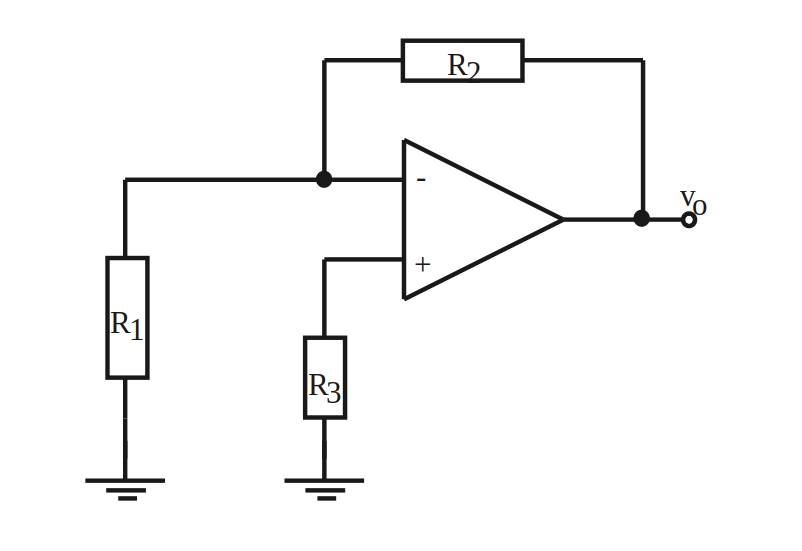
\includegraphics[width=0.6\linewidth]{figuras/op1.png}\\
	\caption{Ejercicio 1.}\label{op1}
\end{figure}


\begin{figure}
	\centering
	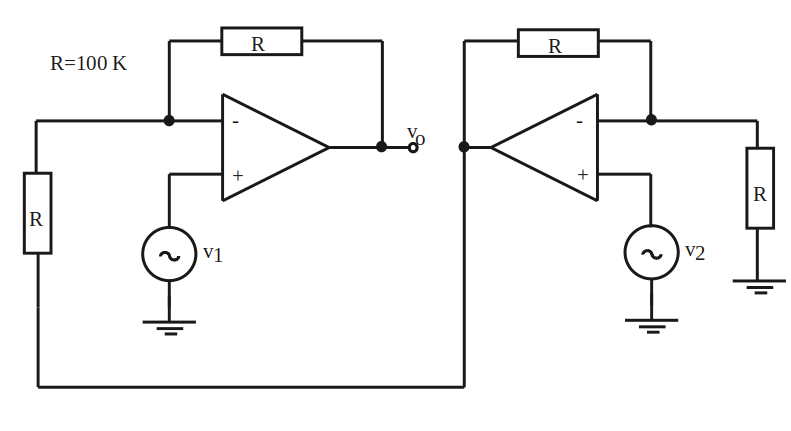
\includegraphics[width=0.6\linewidth]{figuras/op2.png}\\
	\caption{Ejercicio 2.}\label{op2}
\end{figure}


\begin{figure}
	\centering
	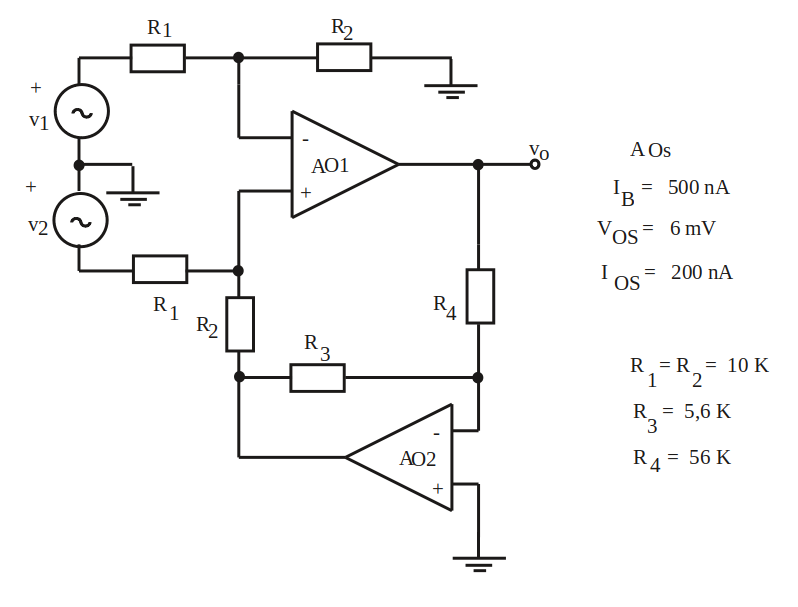
\includegraphics[width=0.8\linewidth]{figuras/op3.png}\\
	\caption{Ejercicio 3.}\label{op3}
\end{figure}


\begin{figure}
	\centering
	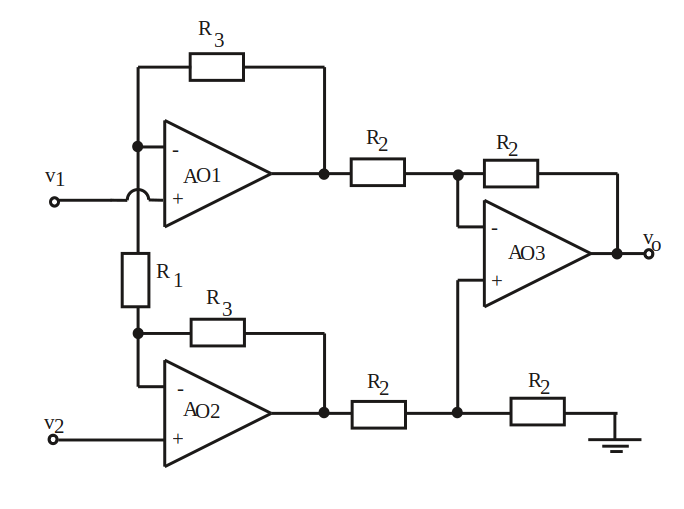
\includegraphics[width=0.6\linewidth]{figuras/op4.png}\\
	\caption{Ejercicio 4.}\label{op4}
\end{figure}

\begin{figure}
	\centering
	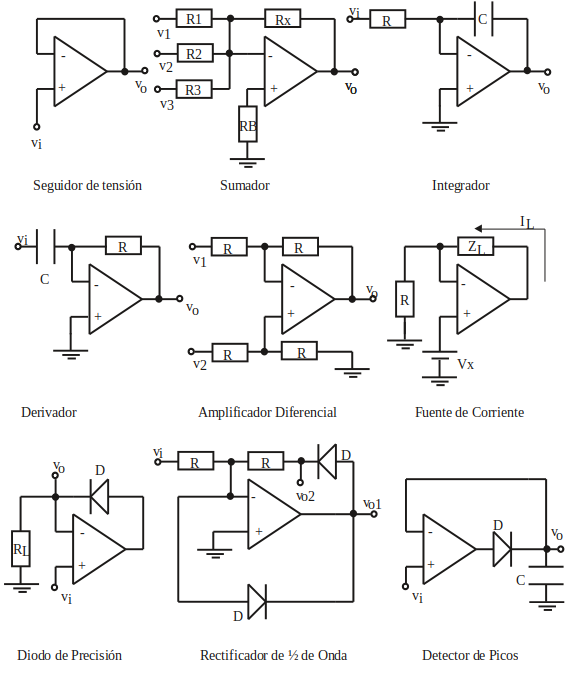
\includegraphics[width=0.8\linewidth]{figuras/op5.png}\\
	\caption{Ejercicio 5.}\label{op5}
\end{figure}

\begin{figure}
	\centering
	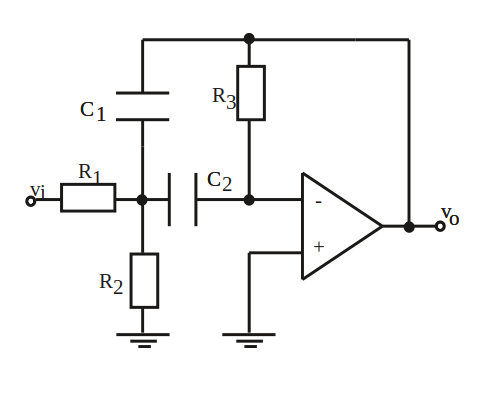
\includegraphics[width=0.6\linewidth]{figuras/op6.png}\\
	\caption{Ejercicio 6.}\label{op6}
\end{figure}

\begin{figure}
	\centering
	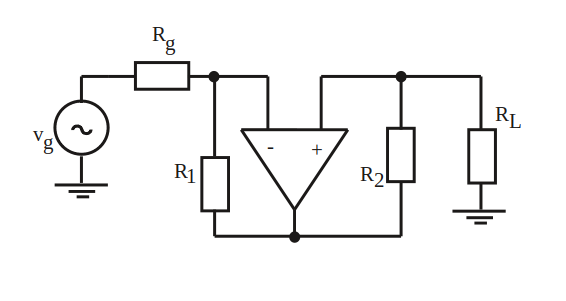
\includegraphics[width=0.6\linewidth]{figuras/op7.png}\\
	\caption{Ejercicio 7.}\label{op7}
\end{figure}

\begin{figure}
	\centering
	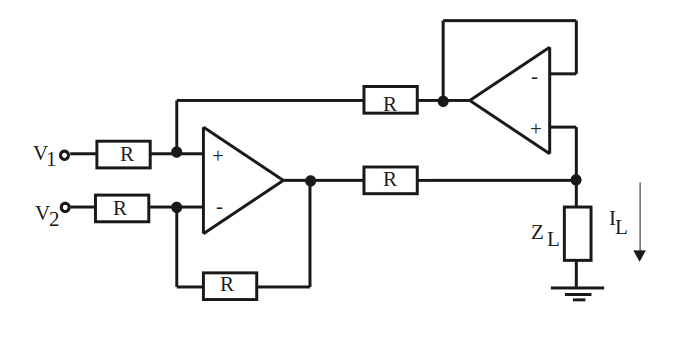
\includegraphics[width=0.6\linewidth]{figuras/op8.png}\\
	\caption{Ejercicio 8.}\label{op8}
\end{figure}

\begin{figure}
	\centering
	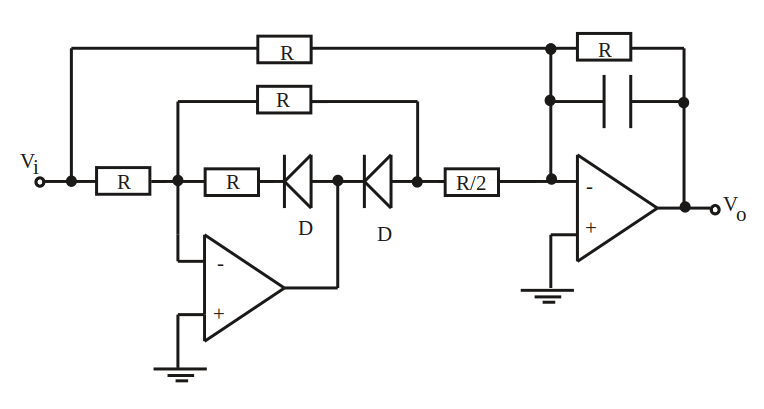
\includegraphics[width=0.6\linewidth]{figuras/op9.png}\\
	\caption{Ejercicio 9.}\label{op9}
\end{figure}

\begin{figure}
	\centering
	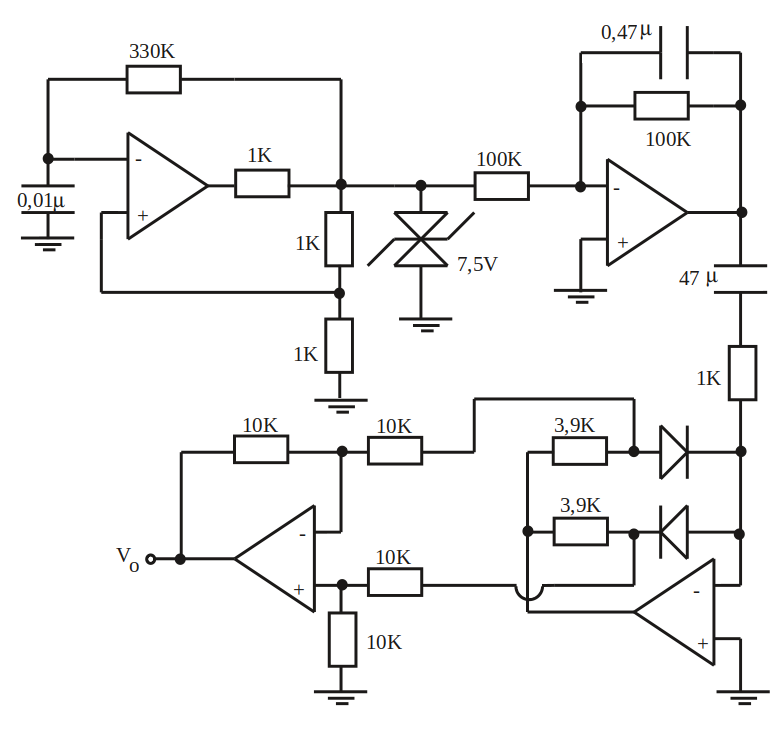
\includegraphics[width=0.8\linewidth]{figuras/op10.png}\\
	\caption{Ejercicio 10.}\label{op10}
\end{figure}


\begin{figure}
	\centering
	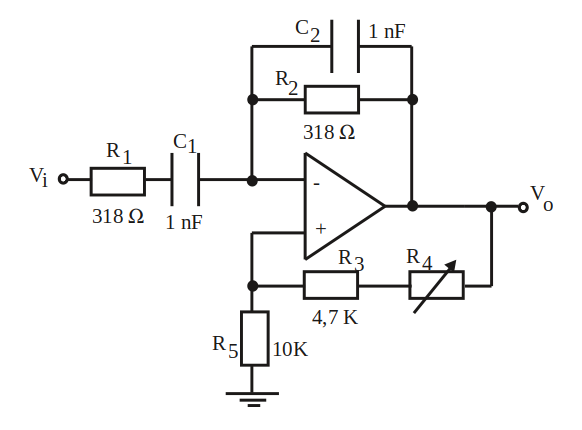
\includegraphics[width=0.8\linewidth]{figuras/op11.png}\\
	\caption{Ejercicio 11.}\label{op11}
\end{figure}


\begin{figure}
	\centering
	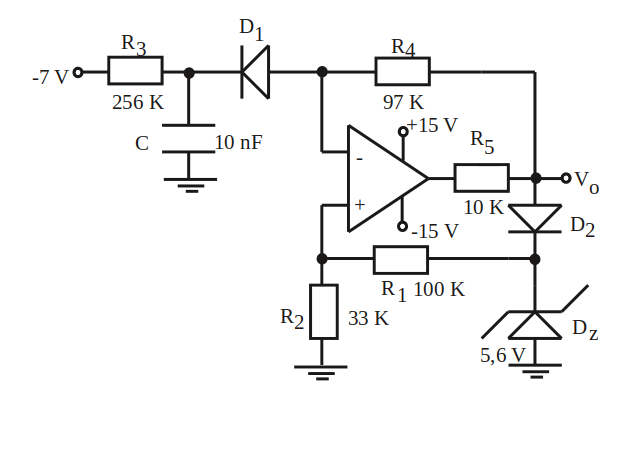
\includegraphics[width=0.8\linewidth]{figuras/op12.png}\\
	\caption{Ejercicio 12.}\label{op12}
\end{figure}



\begin{figure}
	\centering
	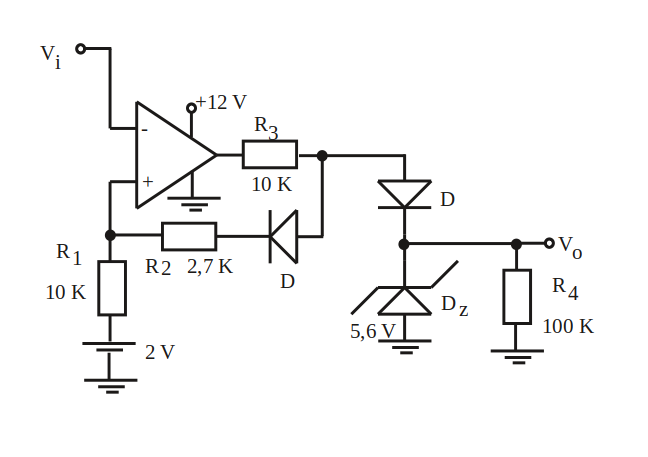
\includegraphics[width=0.8\linewidth]{figuras/op13.png}\\
	\caption{Ejercicio 13.}\label{op13}
\end{figure}


\begin{figure}
	\centering
	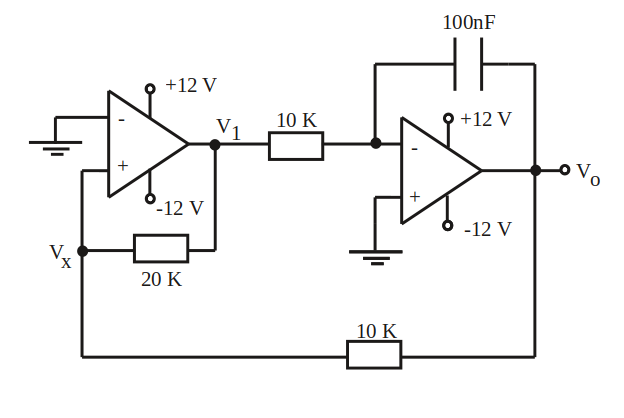
\includegraphics[width=0.8\linewidth]{figuras/op14.png}\\
	\caption{Ejercicio 14.}\label{op14}
\end{figure}
